\chapter{Tests}\label{chap:tests}
Testing of an ADS is challenging as it is difficult to replicate the space environment on Earth. Therefore a lot of testing of ADS relay heavily on simulations. Simulation on the other hand have their own problems as there is a limit on how accurate they can be and they will never truly repentance the system they are simulating. In this chapter the different methods and work flow that was used for testing the MOVE-II ADS will be presented. There will be a special focus on the full hardware tests. For a more in depth view of the simulation based methods see \cite{DavidThesis}           

\section{Test Methods}
In general there where four main categories of test conducted to test and verify the MOVE-II ADS. The tests vary in there use of simulations from completely dependent on simulations to using no simulation. 

\begin{itemize}
  \item \textbf{Simulation-only:} The entire ADS is simulated along with all required environmental models, dynamic models and sensor models. Used for tuning of the Kalman filter and as a baseline check for all other tests.   
  \item \textbf{Software-in-the-Loop:} The ADS is implemented in code as it is on the satellite. The ADS is then given data generated by the simulation environment. Allows for good testing of the code to make sure it is implemented in a way that is consistent with the simulated implementation.    
  \item \textbf{Hardware-in-the-Loop:} The ADS code is running on the same micro-controller that is used on the satellite. It still gets sensor data from the simulated environment. Used to check for numerical issues on the micro-controller and to look for issues regarding timing on the micro-controller. The system is now running in real time.    
  \item \textbf{Hardware-only:} The complete ADS is tested. Where real sensor data is used by the micro-controller. The downside is that the sensor data does not necessarily represent how the sensor data would look in space as the sensors are not in space. Test the complete system and specifically how the algorithms handle real sensor data.        
\end{itemize}  

In \autoref{fig:workFlow} you can see how the different categories influence each other. An important point is how the different test categories influence each other. Where all the test categories are uses the results from the other categories as a reality check and to specify exactly what kind of scenarios should be tested. The figure also shows how dependent all the test are on good characterization and understanding of how the sensors work. 

\begin{figure}[tbp]
	\centering
	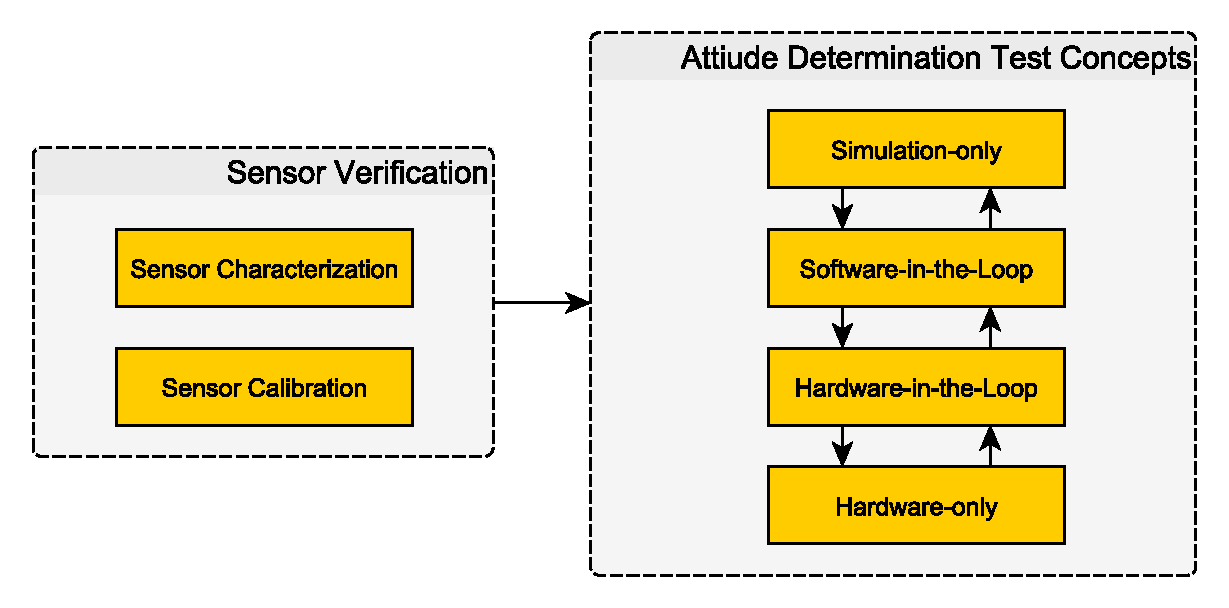
\includegraphics[width=0.7\columnwidth]{./Pictures/testing_concept}
	\caption{Relationshipp between test categories and sensor verification from \cite{DavidThesis}.}
	\label{fig:workFlow}
\end{figure}            

\subsection{Hardware-only}\label{chap:HardwareOnly}
For the Hardware-only test there were four different test cases that were considered, but ultimately only two of them were chosen do there difficulty in execution. All four will be presented before the chosen two will be described in more detail. The two chosen methods where the Algorithm Only approach and the Outdoor test approach.   

\paragraph{Algorithm Only}
The Algorithm Only approach is based around the idea of creating a reference frame around the average of sensor measurements instead of using the reference models as described in \autoref{chap:EKF_MOVE_II}. In other words $\boldsymbol{r}_{mag}$ and $\boldsymbol{r}_{sun}$ are replaced by $\tilde{\boldsymbol{r}}_{mag}$ and $\tilde{\boldsymbol{r}}_{sun}$ respectively and they are defined as in \autoref{eq:avrgLabFrame}. Where $\boldsymbol{b}_i$ and $\boldsymbol{s}_i$ are individual magnetometer and sun sensor measurements respectively.  

\begin{subequations}\label{eq:avrgLabFrame}
\begin{align}
	\tilde{\boldsymbol{r}}_{mag} &= \frac{1}{10}\sum\limits_{i=1}^{10}\boldsymbol{b}_i \\
	\tilde{\boldsymbol{r}}_{sun} &= \frac{1}{10}\sum\limits_{i=1}^{10}\boldsymbol{s}_i 
\end{align}	
\end{subequations}  

The overview shown in \autoref{fig:ADS_overview} can then be modified to reflect this changes as shown in \autoref{fig:outdoorOverview}. The main advantage of this method is that it allows for the testing of ADS with real sensor data without the need for creating a realistic space environment as the models are not used. This method also has some history within the MOVE-II as a similar approach has been used for initial testing earlier \cite{DavidThesis}. 

\begin{figure}[tbp]
	\centering
	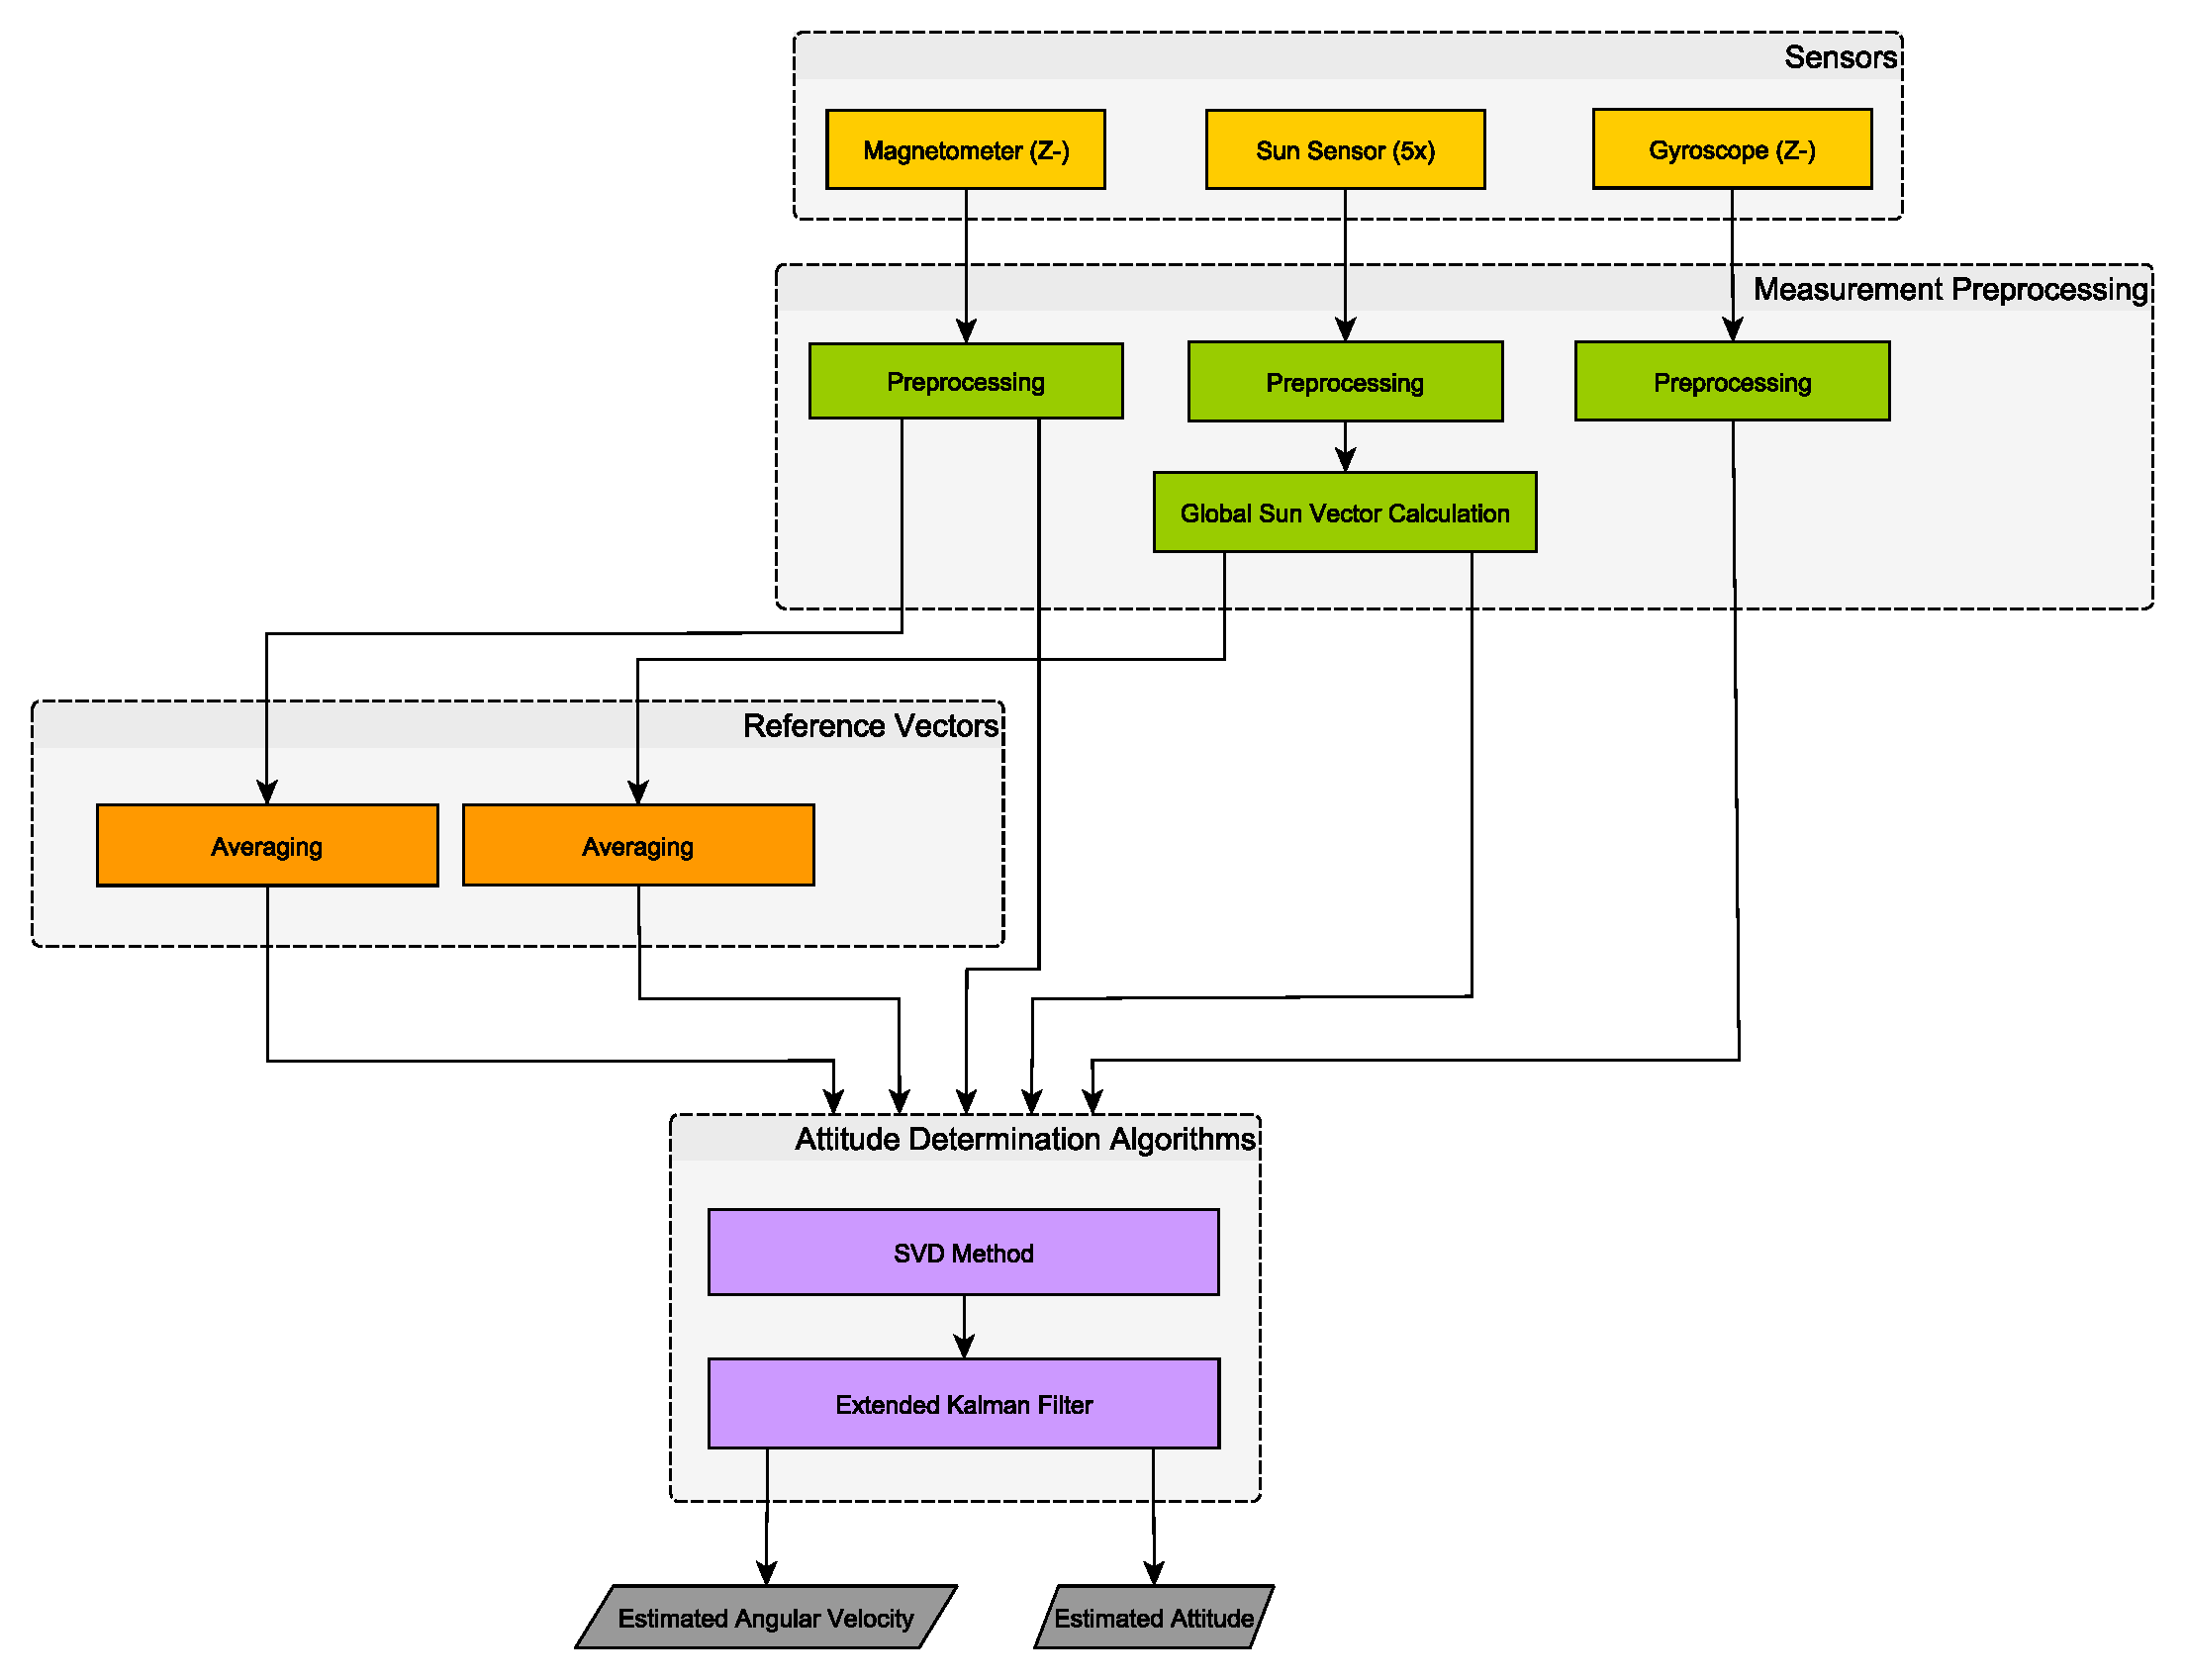
\includegraphics[width=0.7\columnwidth]{./Pictures/ATTDET_Architecture_Ao}
	\caption{An overview of the ADS system when conducting the Algorithm Only test from \cite{DavidThesis}.}
	\label{fig:outdoorOverview}
\end{figure} 

\paragraph{Helmholtz-Cage Approach}
The Helmholtz-cage approach uses a Helmholtz-cage to generate a magnetic field similar to the on expected in the orbit of MOVE-II. The satellite can then be positioned in such a way that the top panel will point directly at a light source representing the sun. As shown in \autoref{fig:Helmholtz-Cage}. By having the top panel face directly at the sun it will be similar to the situation of the satellite having achieved perfect sun pointing. As such all the reference models can be used. This approach has the advantage that none of the firmware has to be changed. The problem is achieving this setup. There is a great uncertainty surrounding the precision of the Helmholtz-cage at the LRT and it is not certain that the cage is able to produce the required magnetic field with an acceptable error. There is also currently no good way of synchronizing the magnetic field model on the satellite and the one used by the Helmholtz-cage to decide what magnetic field to set up. Without this synchronization the test can not be executed. 

\begin{figure}[tbp]
	\centering
	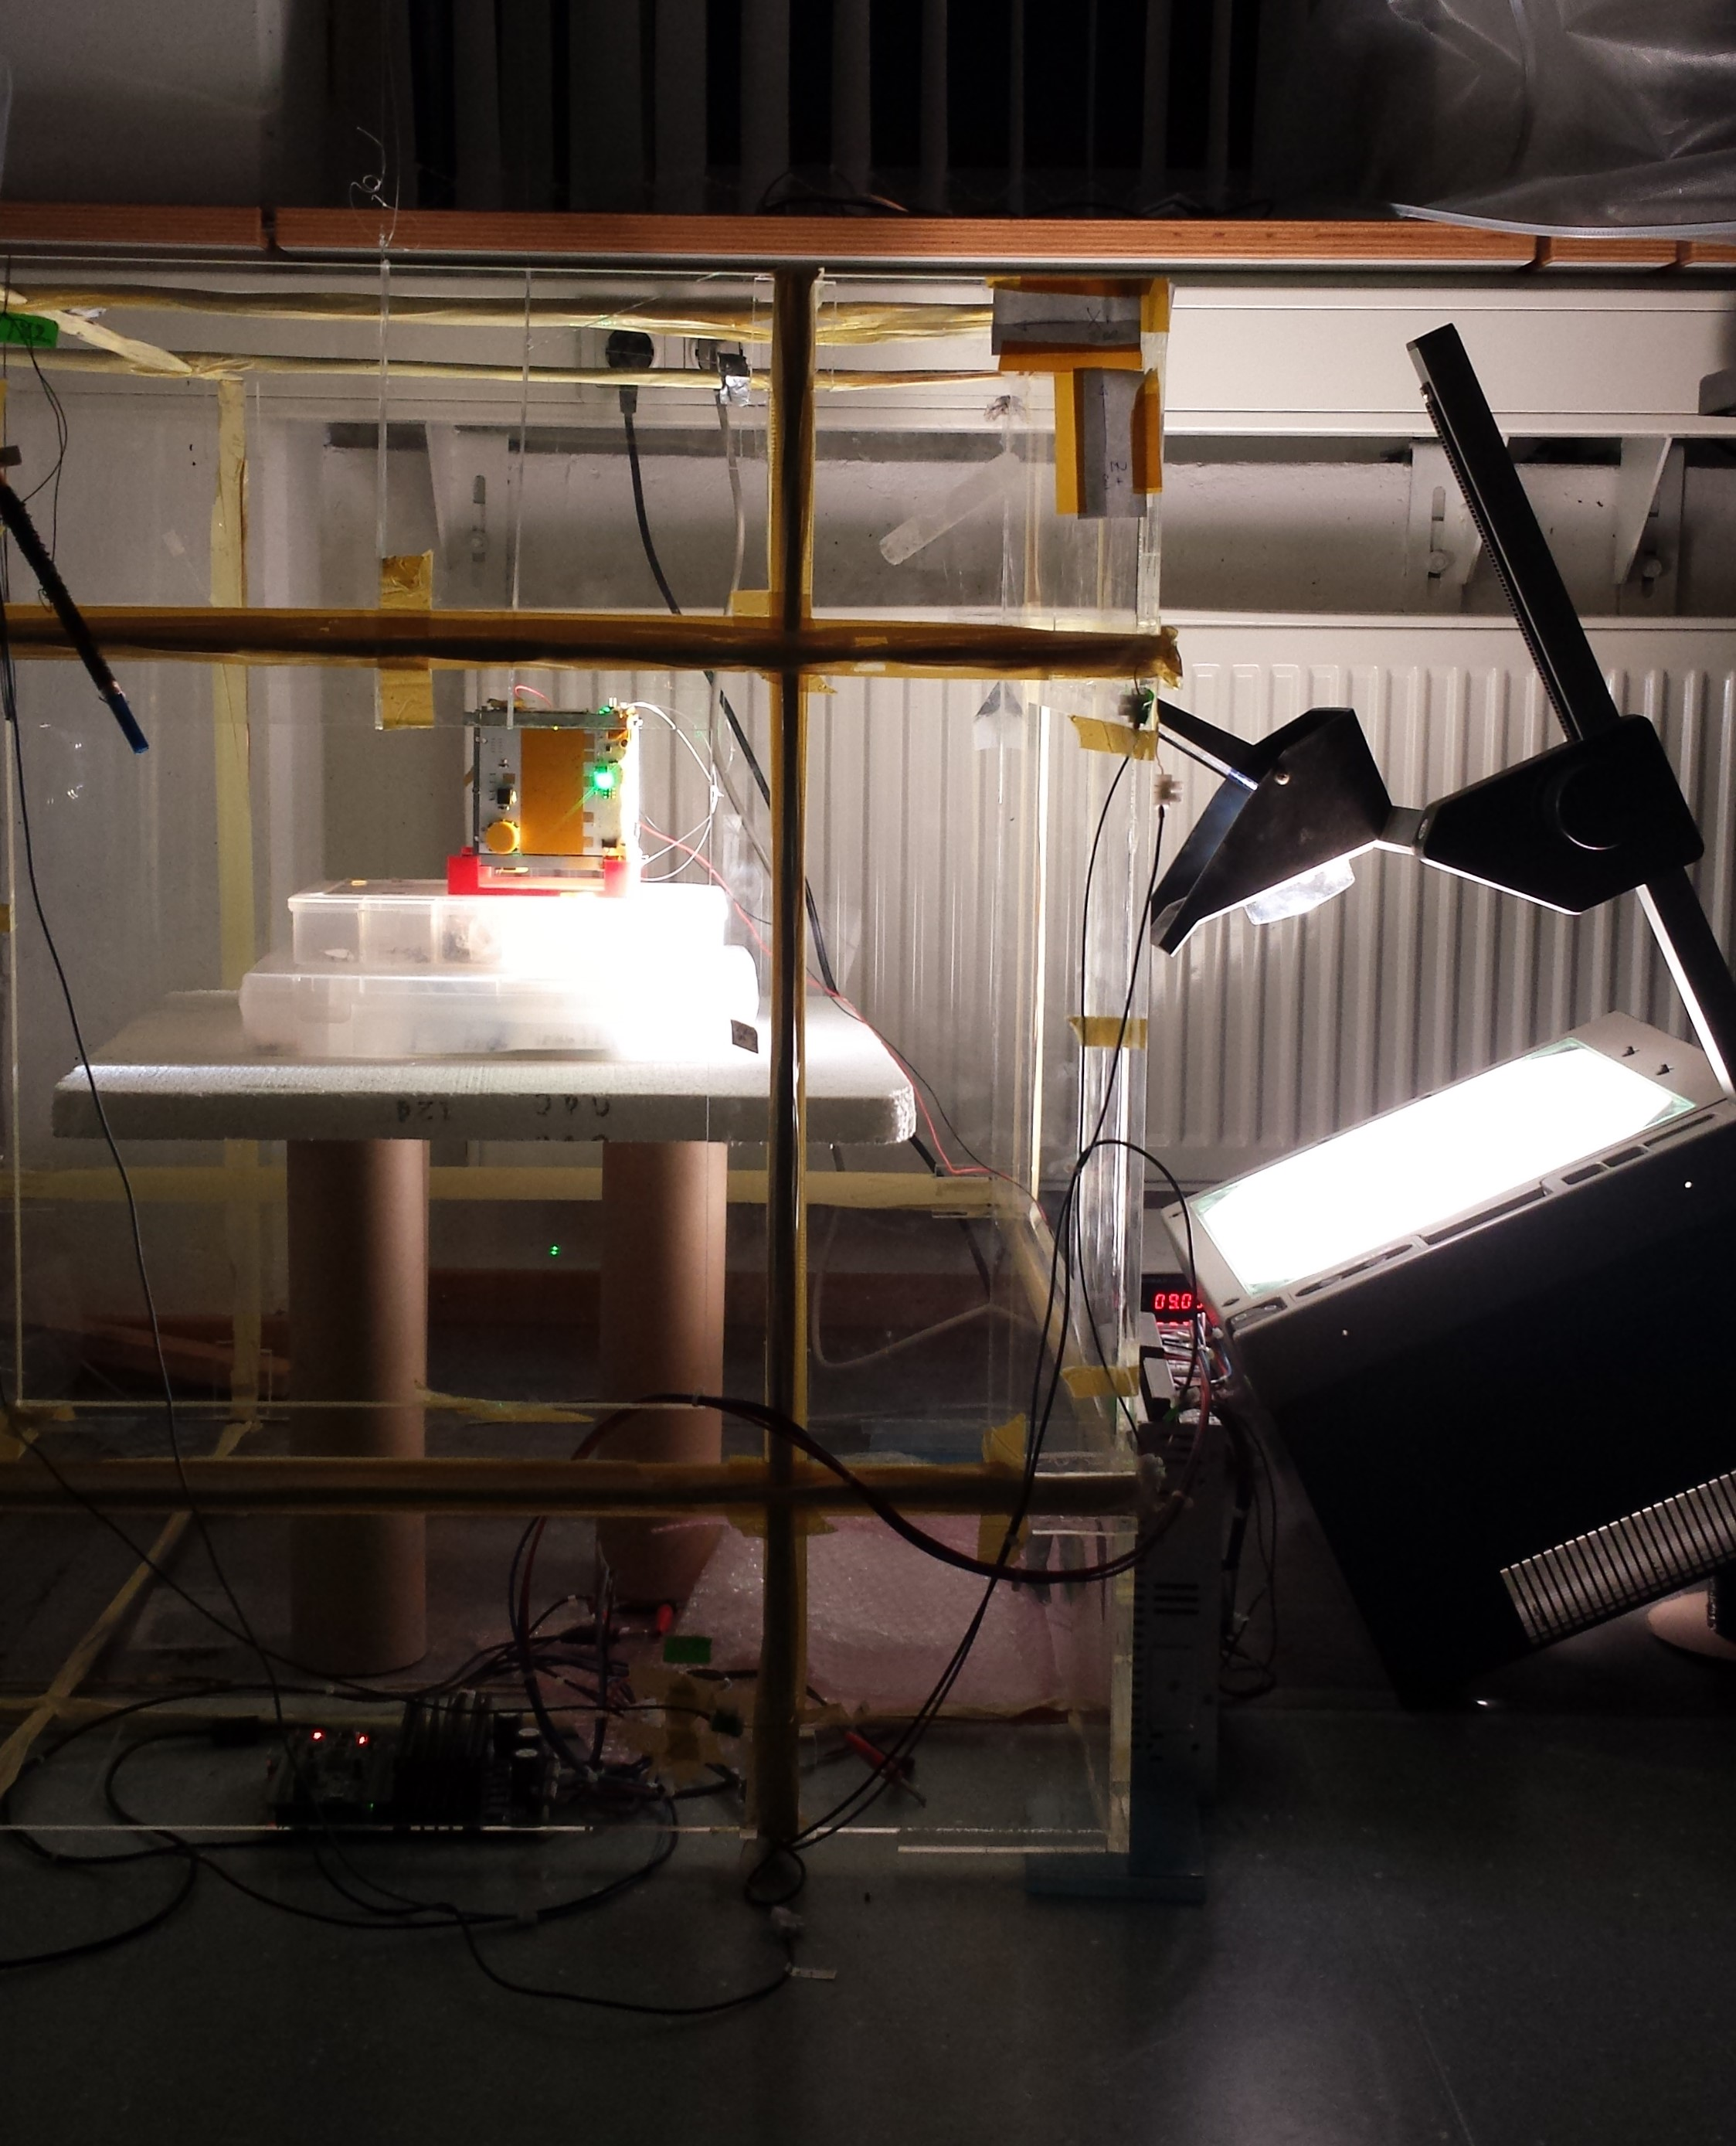
\includegraphics[width=0.3\columnwidth]{./Pictures/Helmholtz_night}
	\caption{Satellite positioned in Helmholtz-cage for ADS testing \cite{DavidThesis}.}
	\label{fig:Helmholtz-Cage}
\end{figure}               

\paragraph{Outdoor}
The outdoor test is simply to take the satellite out on a sunny day. Using the earths magnetic filed and the sun as inputs to the sensors. As both the magnetic field model and sun position model also works for positions on earth the models can be used. Some care has to be taken in choosing a spot with little magnetic disturbance. Some firmware changes are necessary for this test. First of all the satellite is not moving relative to the ECEF frame any more. So the orbit propagator needs to be disabled and a constant position has to be give to the IGRF. Leading to an overview of the ADS as shown in \autoref{fig:outdoorOverview}. The position of the satellite also has be expressed in the ECEF frame. This test has the advantage that it uses almost the entire ADS system. Especially important it that it test all reference models acting with real sensor data. A big disadvantage of this test is that it requires substantial effort to set up as all the equipment has to be brought outside. Also it is reliant on good weather. All this factors makes it unsubtle for intensive debugging, but a good test to test large parts of the system working together.         

\begin{figure}[tbp]
	\centering
	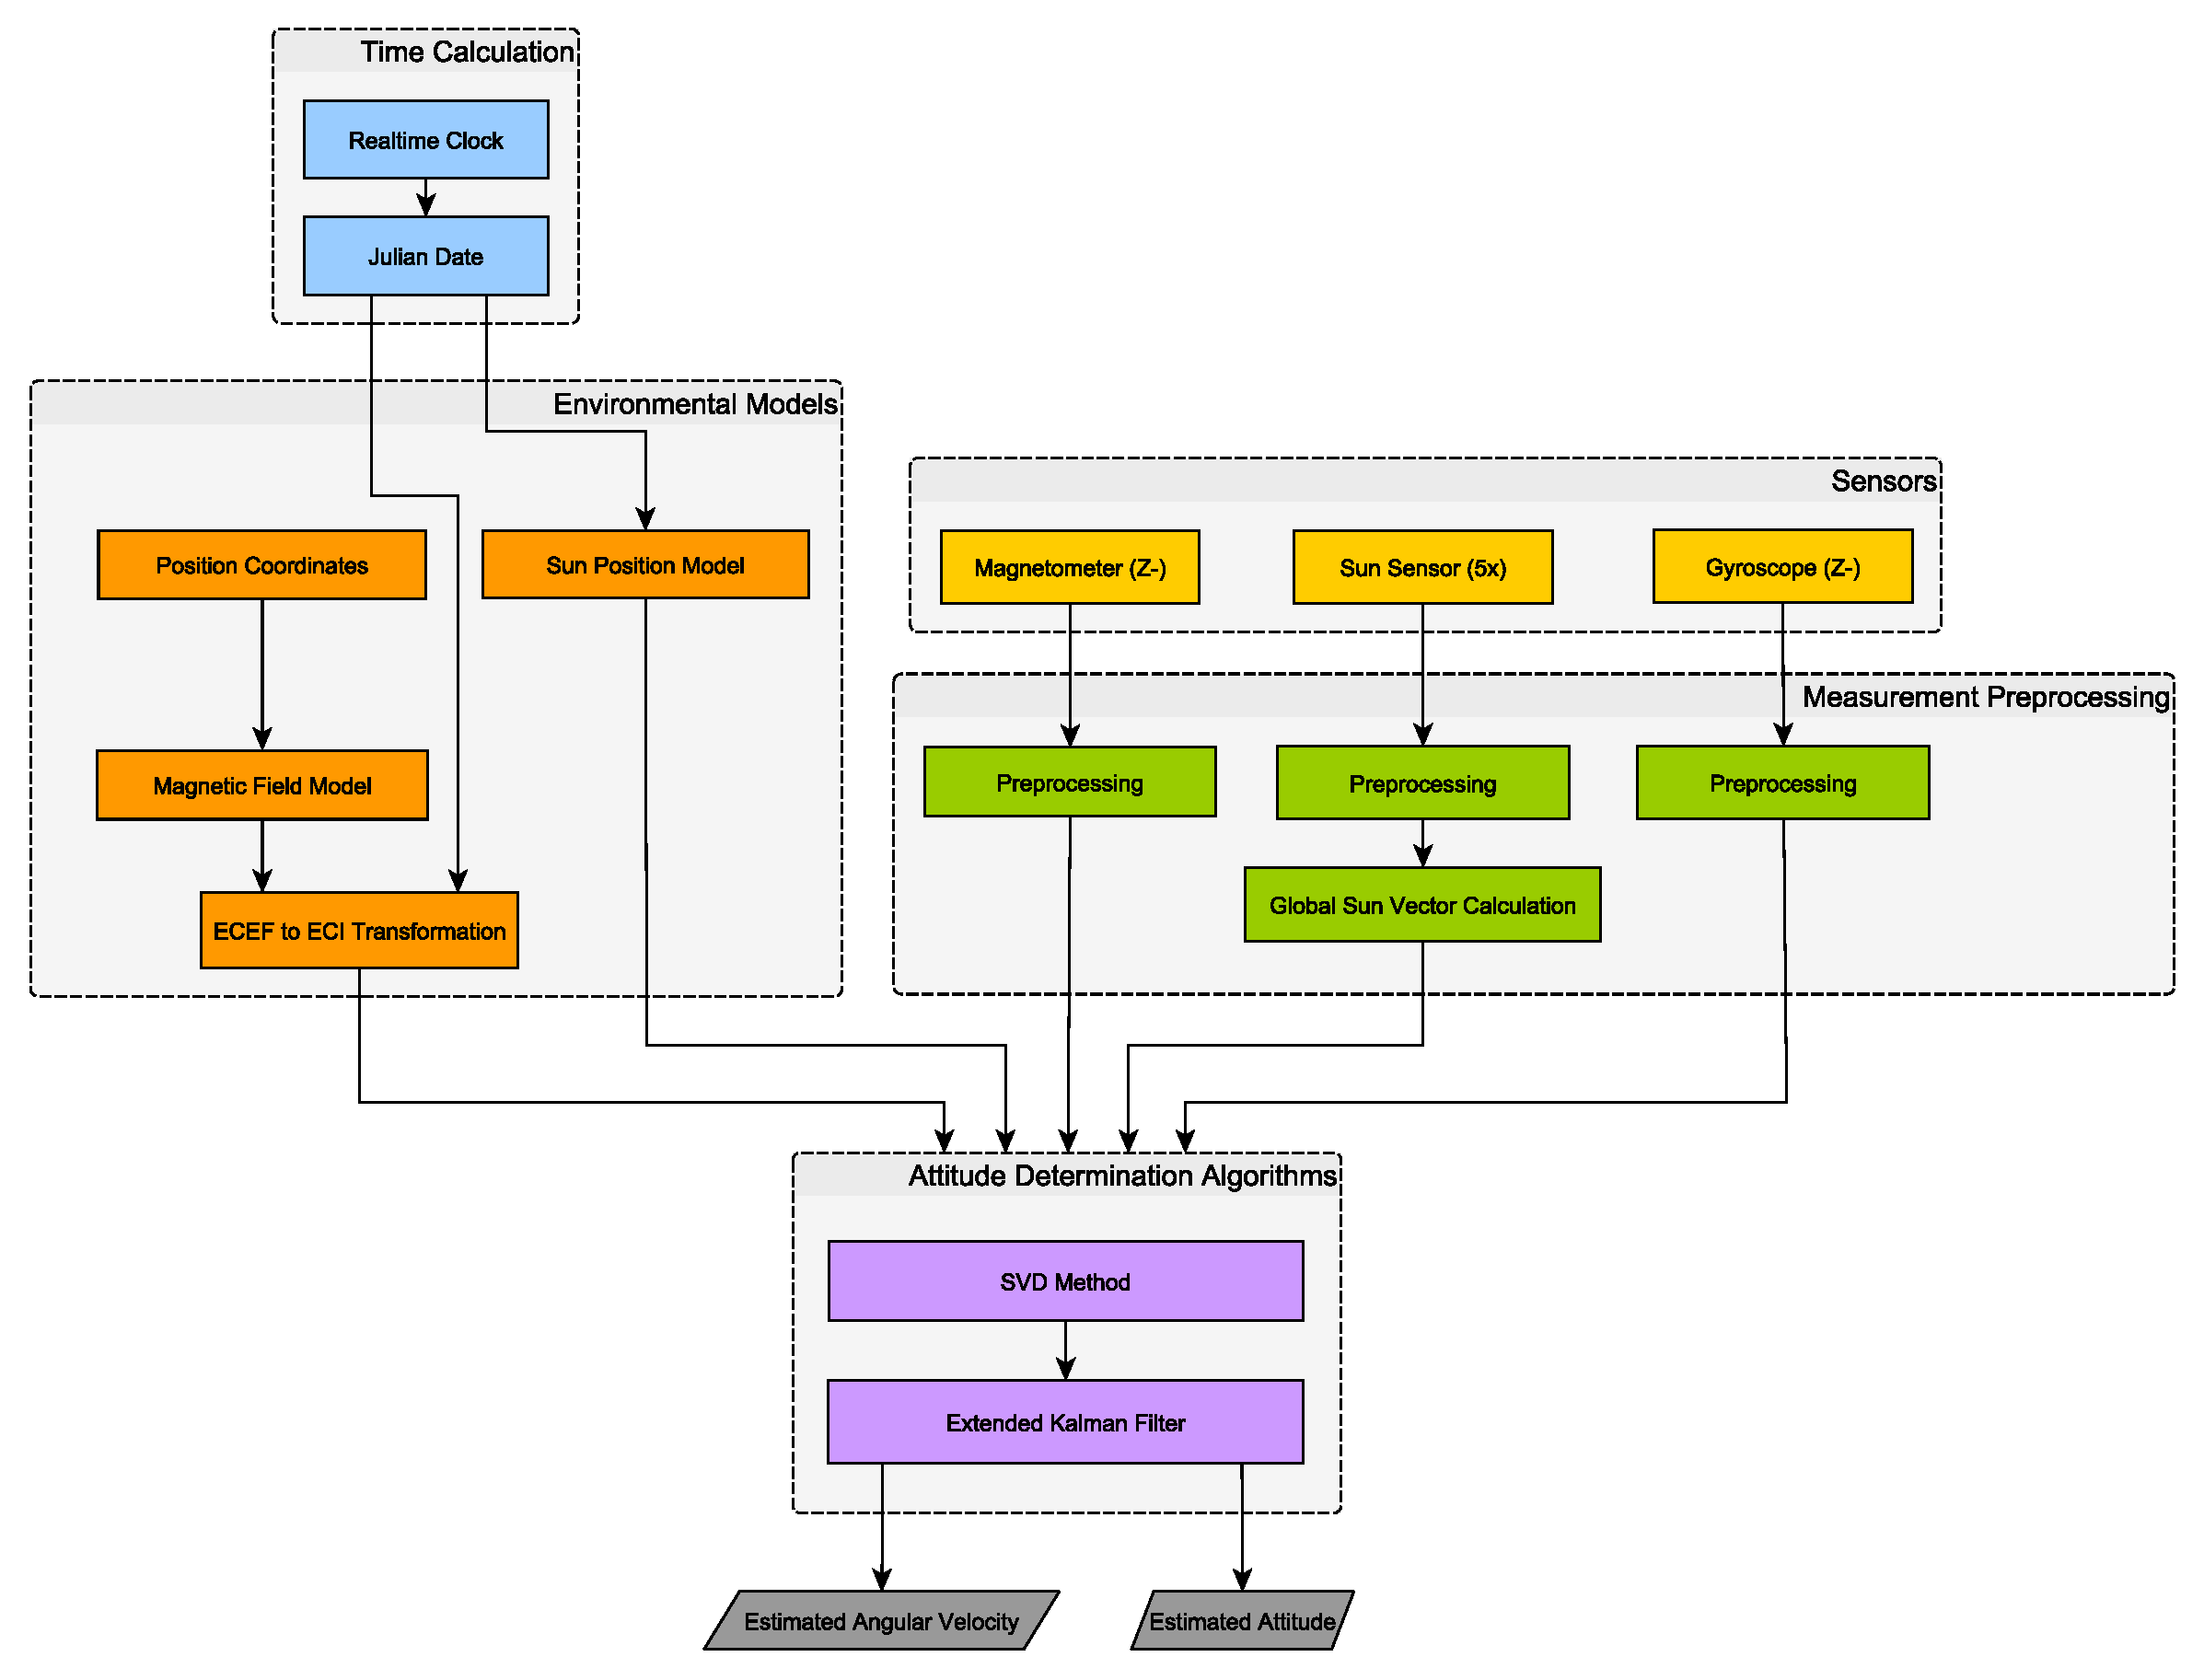
\includegraphics[width=0.5\columnwidth]{./Pictures/ATTDET_Architecture_O}
	\caption{Overview of the ADS when conducting the Outdoor test from \cite{DavidThesis}.}
	\label{fig:outrdoorOverview}
\end{figure}

\paragraph{UWE-3 Laboratory Approach}
The UEE-3 laboratory approach is described in \cite{UWE-3}. The test requires a turntable, Earth's magnetic field and a suitable light source representing the sun. The main idea is to place the light source a suitable place in the laboratory and then adjust the time on the satellite so the position of the light source will be consistent with the reference models of the sun position. This works because the position of the sun is only depends on time so any reasonable position of the light source should also be a position of the sun in the sun position model given the right time. To find this time a matching algorithm was developed by the UWE-3 team it calculates the time based on the three measurements light source elevation angel, angel between magnetic field and light source and the azimuth of the light source. This approach was not chosen because there was no access to a suitable light source and the time investment to develop the algorithm to find the right time was considered to large.

\subsection{Implementation}
The tests where first and primarily implemented on what is called the PrintSat before they were tested on the Flight Model (FM). The PrintSat is described in more detail later in this section. The PrintSat was primarily used because it is a lot easier work with and is more readily available to the ADCS team as it belongs to the team. It is also more suitable for experimenting as it is not as critical if the PrintSat breaks.     

\paragraph{PrintSat}
The PrintSat is a test satellite developed by the ADCS team of MOVE-II. It only contains the elements of the satellite relevant for the ADCS and have been used extensively for testing various parts of the ADCS. The PrintSat contains all the panels that make up that ADCS system, namely the four side panels, the top panel and the main panel. So functionally it has all the same functionality as the ADCS on the FM. The panels are hold together in a cube like construction shown in \autoref{fig:printsat}. In addition the to the ADCS element the PrintSat also contains a beaglebone that is used to represent the main computer on the satellite and the power supply. The beaglebone and the ADCS communicate over SPI in the same way that the ADCS communicates with the rest of the satellite on the FM. This means the ADCS on the PrintSat can be controlled with commands in the same way as on the FM. There also exists an UART connection between the beaglebone and the ADCS that allows additional data to be recorded when using the PrintSat. The power supply also contains a battery so the PrintSat can function with out an external power source. In addition the beaglebone contains a WiFi unit meaning the PrintSat can be connected to a wireless network and reached over an SSH connection allowing for wireless control of the PrintSat. 

\begin{figure}[tbp]
	\centering
	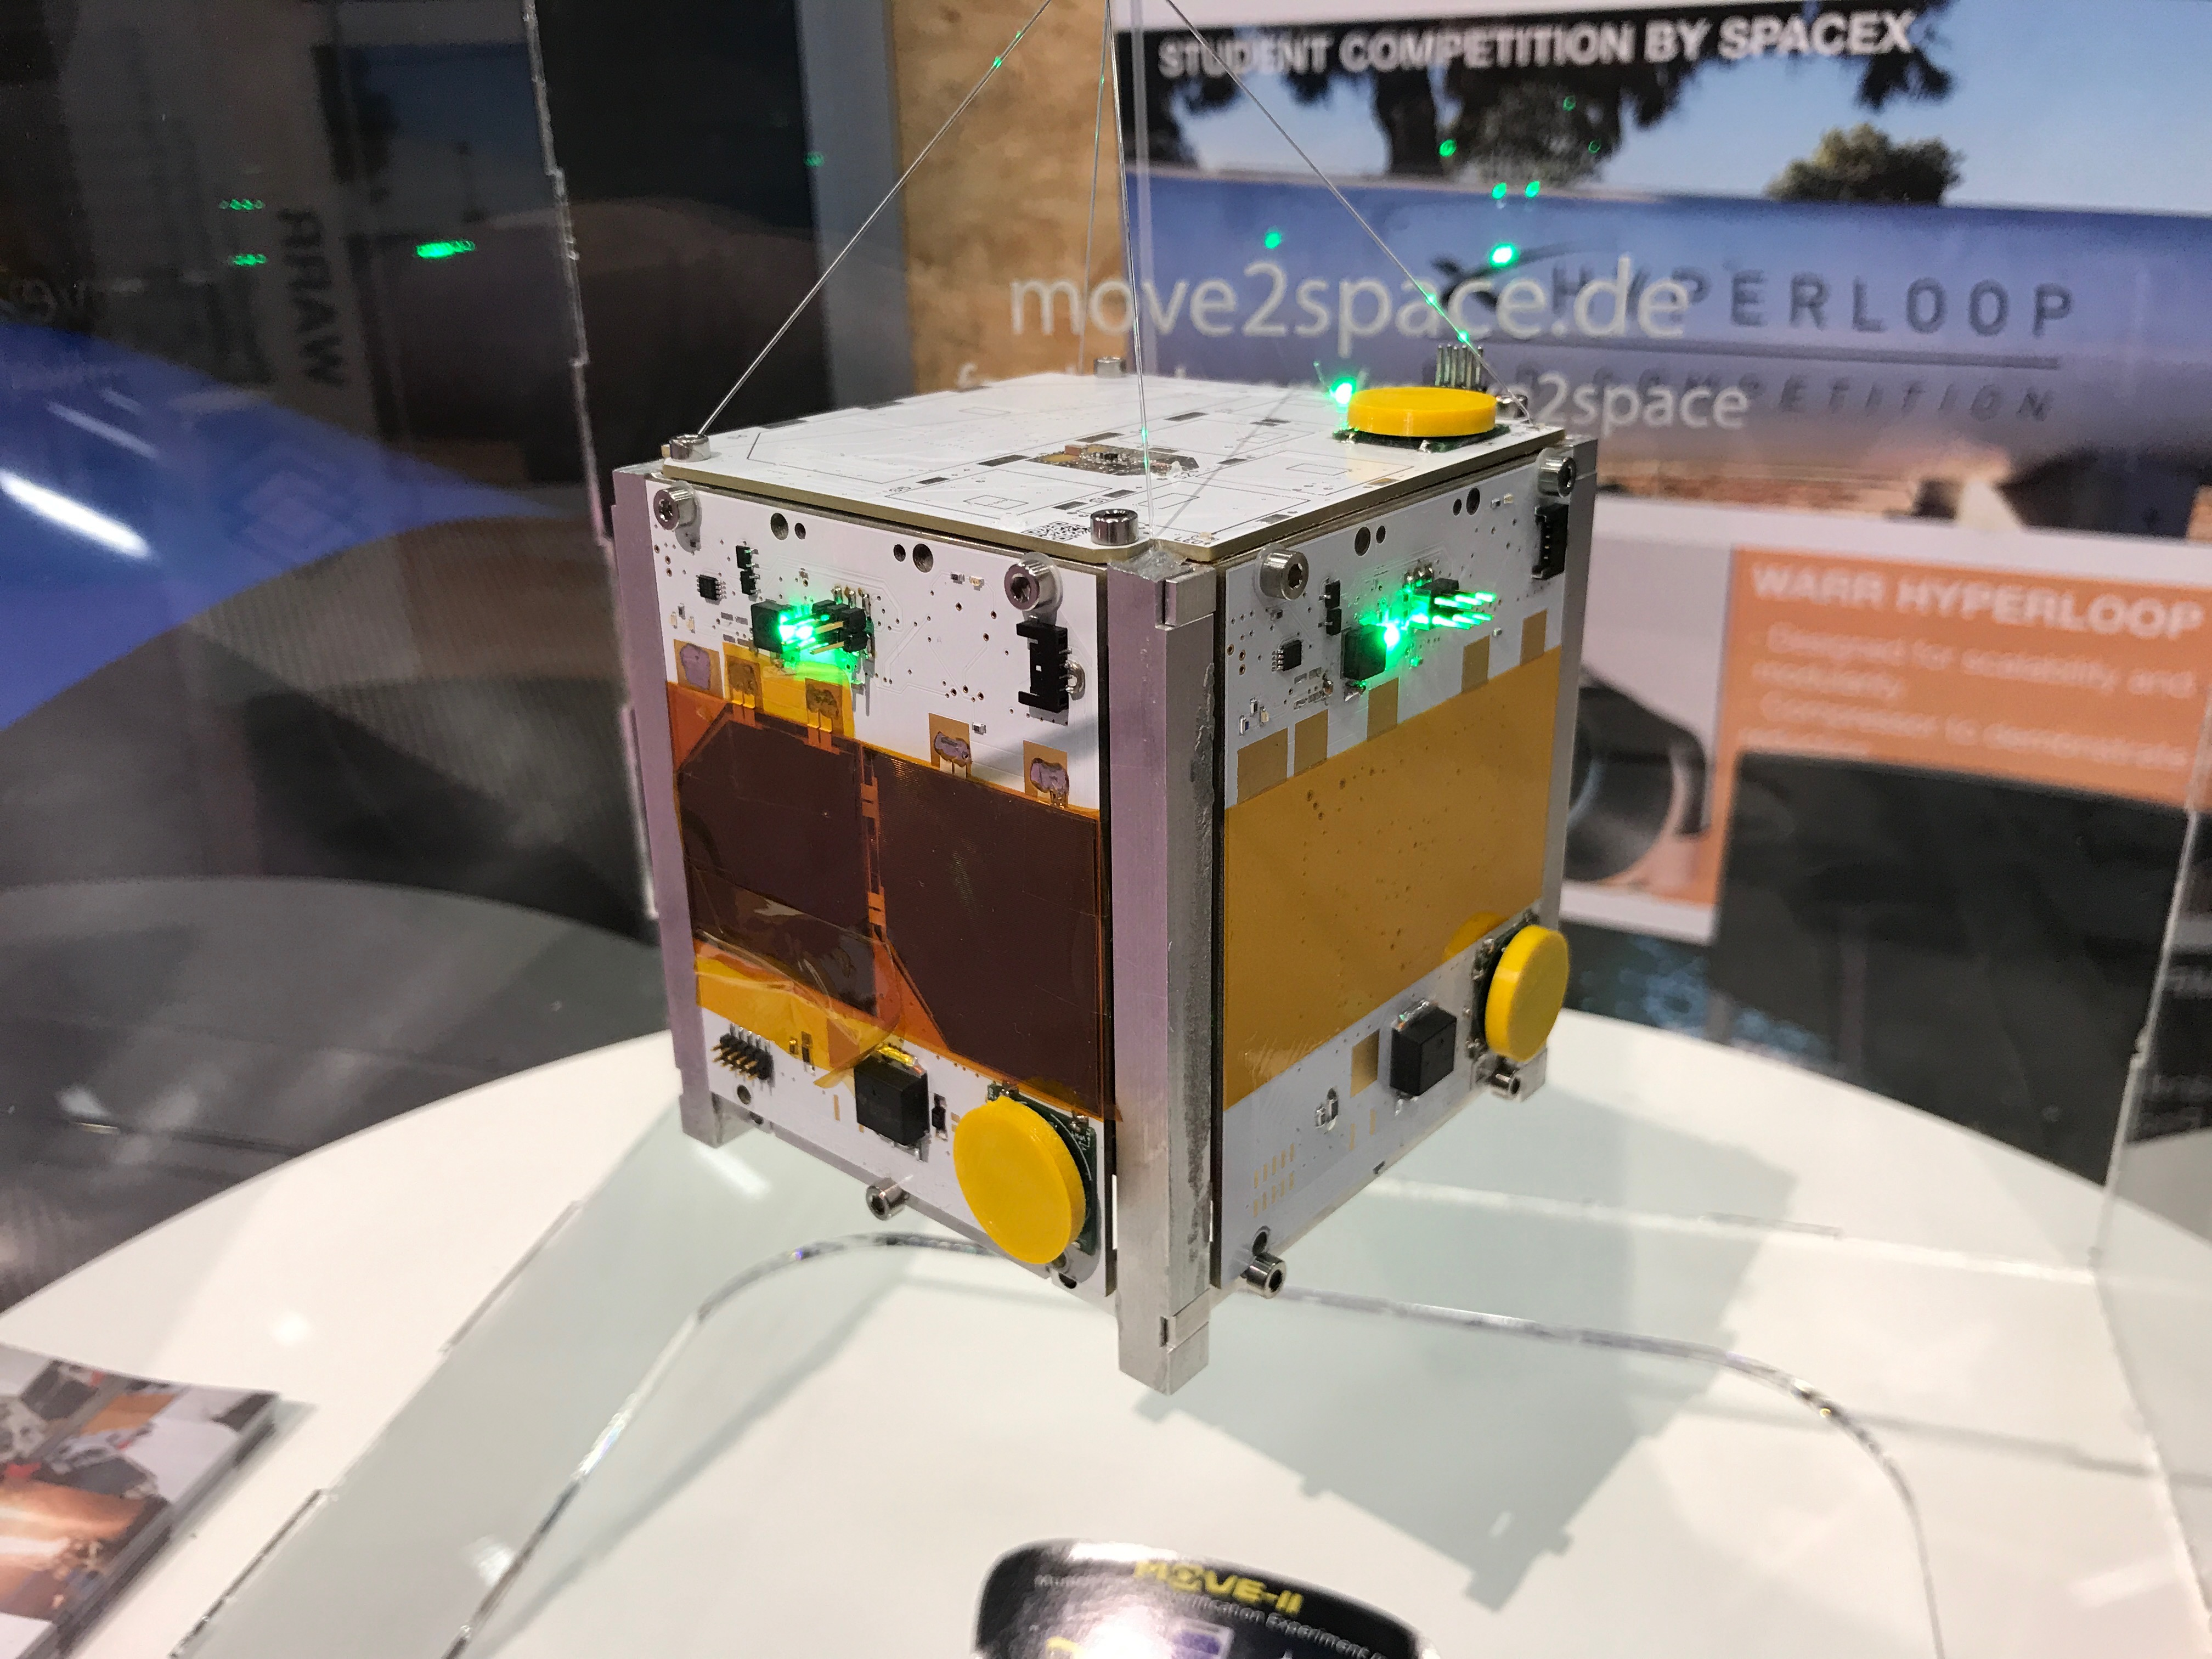
\includegraphics[width=0.5\columnwidth]{./Pictures/printsat2}
	\caption{PrintSat from \cite{DavidThesis}.}
	\label{fig:printsat}
\end{figure}

\subsubsection{Implementation of Algorithm Only}
To implement the Algorithm Only approach some small changes to the ADCS firmware was necessary to disable the reference models and replace them with the averaging function to create the lab frame as described in \autoref{chap:HardwareOnly}. The firmware was also extended with additional debug outputs over a UART connection as the data in the housekeeping files are not sufficient for debugging and proper characterization of the ADS. It should be noted that the data gathered over UART is only accessible on the PrintSat as the FM does not have a UART connection.

The Algorithm Only approach was implemented in a laboratory. A turntable was used to give the satellite a known rotation. The approach also requires a light source. For the light source an overhead projector was used. The overhead projector has been used in previous test of the ADCS. A picture of the test setup can be seen in \autoref{fig:AlgorithmOnlyTestSetup}. With the turntable and the overhead projector different variations can of the test can be set up. Where the variations include static or rotating test with our with out light. Where with light represents when the satellite is in sun and no light represents when the satellite is in the shadow side of the Earth. 

\begin{figure}[tbp]
	\centering
	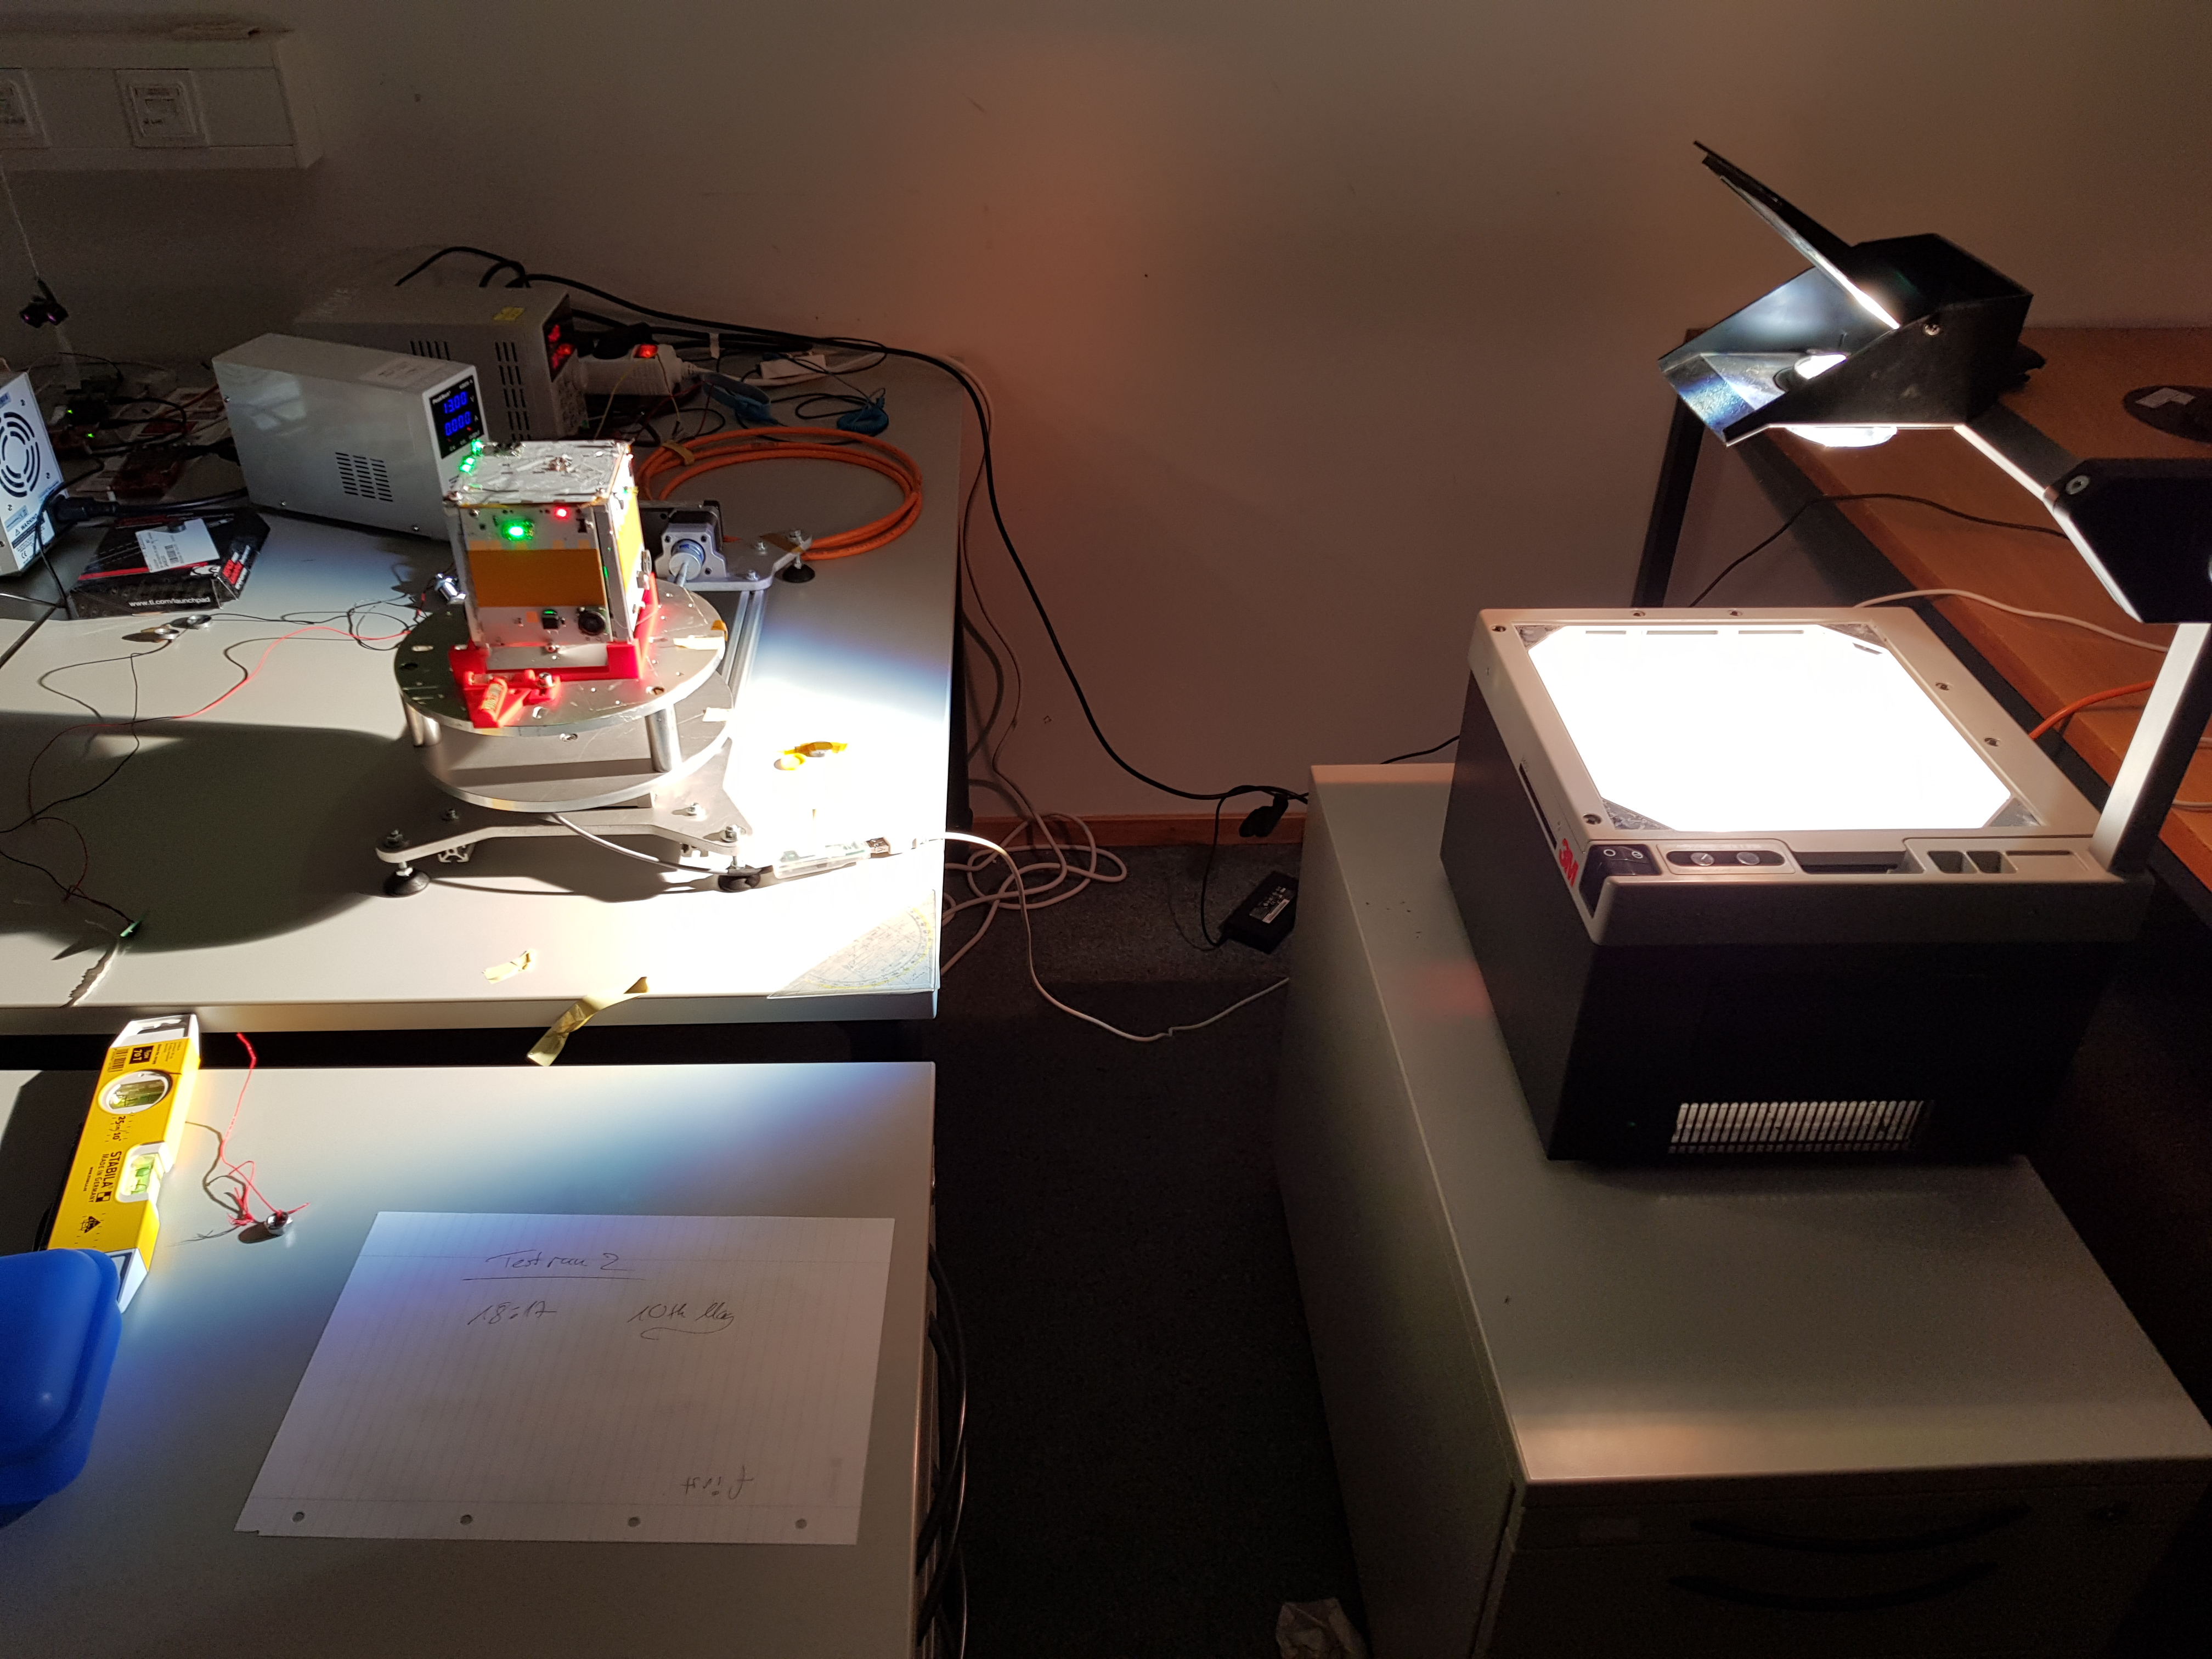
\includegraphics[width=0.5\columnwidth]{./Pictures/Indoor}
	\caption{Algorithm Only setup with the PrintSat from \cite{DavidThesis}.}
	\label{fig:AlgorithmOnlyTestSetup}
\end{figure} 

Before the tests where started the turntable where leveled using a water level. Once the satellite was leveled the recording service both for housekeeping data and the data transmitted from the ADCS to the beaglebone over UART is started. The satellite was then put in attitude determination (ATTDET) mode. The satellite is stationary for some time to generate the new reference frame, after that the turntable can start to turn if it is a rotating test. It is also a possibility to reinitialize the the EKF parameters during the test. After the test the recorded data can be transfered from the PrintSat to a PC for post processing. The time when the turntable is started and stopped is also recorded so it is possible to recreate the rotation of the turntable to have a reference to compare the estimated quaternion with. 

\subsubsection{Implementation of Outdoor}
For the outdoor approach some changes to the firmware had to be implemented. The propagator had to be disabled and a constant position had be be given to the IGRF model. It was also necessary to do some more changes to the debug output and the housekeeping data. This is because the output from the ADS when all models are used is the quaternion representing the rotation between ECI and body-fixed frame. This data is hard to interpret, so a new frame was defined. This frame called the lab frame is defined as North East Down (NED) so the x-axis points north, the y-axis points east and the z-axis completes the right hand rule by pointing down towards the earth. This frame is much easier to analyze as it is easy to align the fixed-body frame with the lab frame. To get the quaternions to represent the rotation between the lab frame and the fixed-body frame a simple transformation is needed. In the ADS there already exist a function to go from ECI to ECEF frame. The transformation between ECEF and the lab frame can be accomplished by the rotation matrix shown in \autoref{eq:ECEFtoLab} according to \cite{UWE-3}. Where $\Phi$ is latitude and $\lambda$ is longitude of the position where the test is conducted. The decision to do this calculations live on the satellite instead of in post processing was mainly due to the fact that the ECI to ECEF transformation is time dependent and it would be difficult to get the synchronization correct.    

\begin{equation}\label{eq:ECEFtoLab}
	\boldsymbol{R}_{LE} = \begin{bmatrix}
		-sin(\Phi)cos(\lambda) & -sin(\Phi)sin(\lambda) & cos(\Phi) \\
		-sin(\lambda) & cos(\lambda) & 0 \\
		-cos(\Phi)cos(\lambda) & -cos(\Phi)sin(\lambda) & -sin(\Phi) \\
	\end{bmatrix}
\end{equation}                       

In the execution of the actual test the satellite and turntable was brought out to a nearby field away from buildings. A WiFi router that could be powered with a micro-usb cable from a computer was also brought. This was to create a local WiFi network so commands could be send to the PrintSat. The body frame of the satellite was then aligned as good as possible to the lab frame. This was done by using a water level to level the satellite and by using a simple compass to align the x-axis of the satellite as good as possible to the north. A picture of the setup can be seen in \autoref{fig:OutdoorTest}. Once the satellite was aligned with the lab frame the data recording services where started before the satellite was put into ATTDET mode. The EKF can also be reinitialized by a simple command. Then the turntable could start turning if it was a rotating test. It should be noted that there are no successful rotation outdoor tests as there was some difficulty getting the turntable to work with the mobile power source. Tests of when the satellite is in the shadow of the Earth can also be conducted by increasing the threshold of the sun sensors to a very high value. This means that none of the recorded sun sensor data will be accepted as valid and will therefore not be used in the EKF. This is similar to what will happen once the satellite is on the shadow side of Earth. It should be noted that for this test setup it is very important that the sensors are properly calibrated and that the time on the satellite is correct. In contrast to the Algorithm only test where calibration and satellite time does not matter.

\begin{figure}[tbp]
	\centering
	\includegraphics[width=0.5\columnwidth]{./Pictures/Outdoor}
	\caption{Outdoor test setup with the PrintSat from \cite{DavidThesis}.}
	\label{fig:OutdoorTest}
\end{figure}

\ifdraft
\section{Test Results}
Only the test result from the Hardware-only test will be presented, to get an overview of the different simulation test see \cite{DavidThesis}. The analysis of the result will also be more qualitative than quantitative. For a more quantitative approach see \cite{DavidThesis}. For the PrintSat there will be result for both the Algorithm only and Outdoor test, for the FM there are only results from the Algorithm only test as it was not possible to conduct an successful Outdoor test before the FM had to be delivered to the launch provider for integration. 

\subsection{PrintSat}
Using the PrintSat with the Algorithm only and Outdoor approach a large portion of the functionality of the ADS has been verified and the confidence in the ADS has increased a lot. The test has also shown some malfunction in the ADS that are currently still under investigation. 

\subsubsection{PrintSat Algorithm Only Results}
The most typical working conditions that the satellite will face in space is spinning with and with out sun light. For those two scenarios the result also look promising. In \autoref{fig:cdr3RotSun} and \autoref{fig:cdr3RotNoSun} you can see the results from a test where the satellite is rotated around it's z-axis three times. Where \autoref{fig:cdr3RotSun} and \autoref{fig:cdr3RotNoSun} is with and with out sun respectively. The dotted lines in the plot is the reference trajectory. The reference trajectory is calculated by rotating a reference quaternion around the z-axis with angular velocity calculated by dividing the total number of revolution by the time taken to couplet the rotations. As you can see from the results both test work reasonably well. The estimated quaternion are able to follow the reference quaternion to an acceptable degree. 

\begin{figure}[tbp]
	\centering
	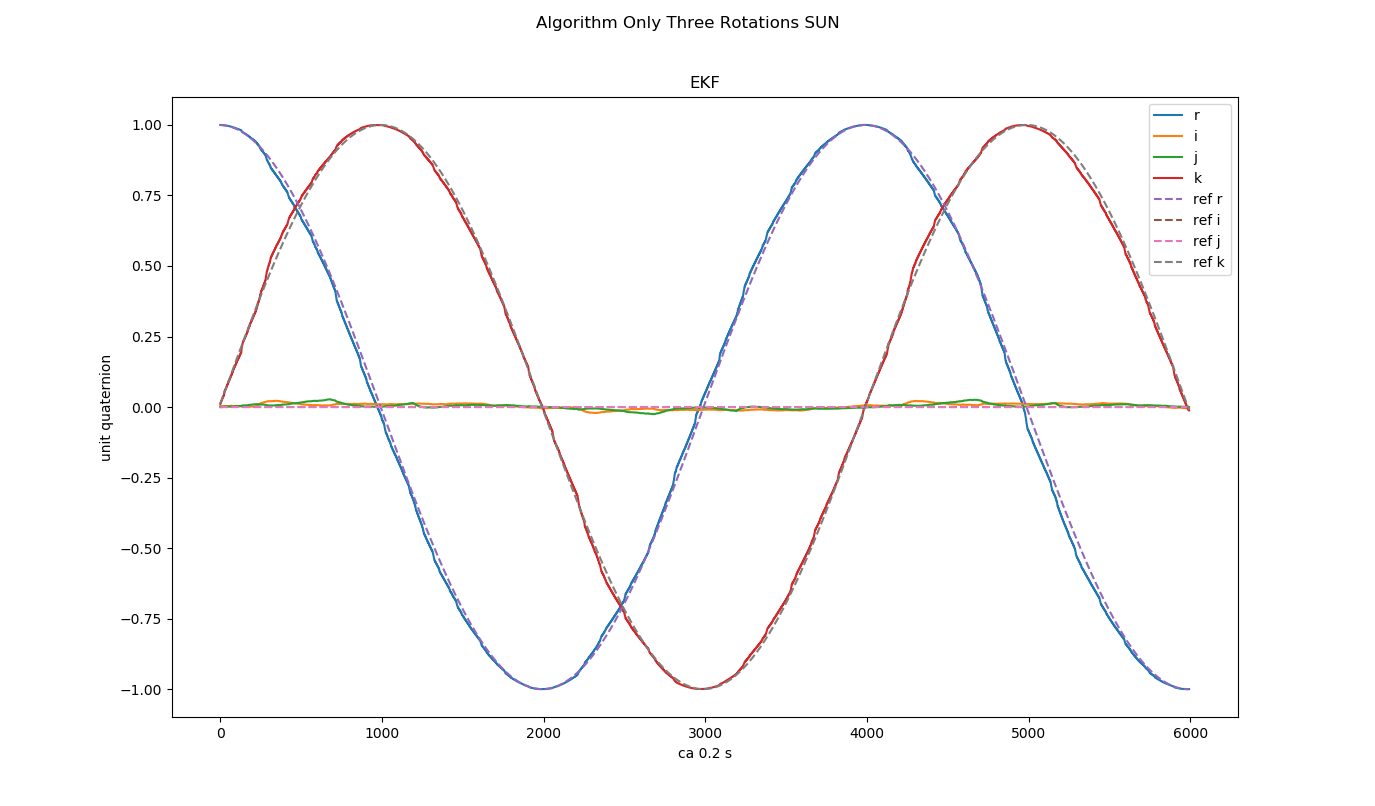
\includegraphics[width=1\columnwidth]{./Pictures/cdrRun3ThreeRotationsSun}
	\caption{Plot of recorded quaternion and reference quaternion for Algorithm only test using the PrintSat. Three rotations with sun}
	\label{fig:cdr3RotSun}
\end{figure}               

\begin{figure}[tbp]
	\centering
	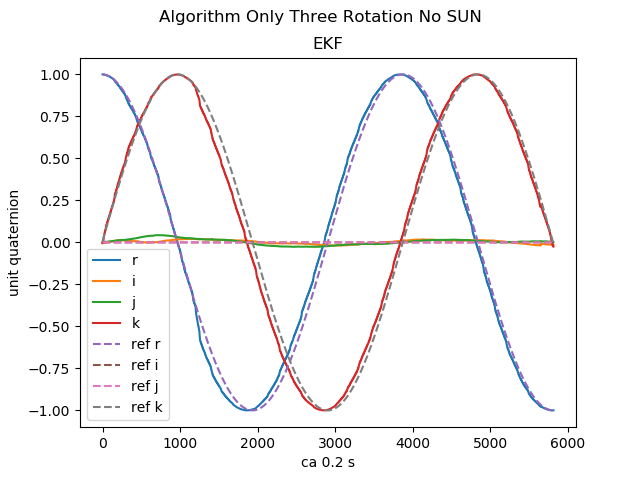
\includegraphics[width=1\columnwidth]{./Pictures/cdrRun3ThreeRotationsNoSun}
	\caption{Plot of recorded quaternion and reference quaternion for Algorithm only test using the PrintSat. Three rotations with  no sun}
	\label{fig:cdr3RotNoSun}
\end{figure}

\subsubsection{PrintSat Outdoor Results}
When conducting the outdoor test there was no possibility of conducting tests with rotations as there was problems getting the turntable to work with batteries. A problem arises when there is no rotation. In \autoref{fig:OutdoorNoRotationSun} which is a test with sun and no rotation it seems to be fine. The recorded quaternion is about $[1 0 0 0]$ which is expected as the PrintSats body-fixed frame is aligned with the lab frame. In \autoref{fig:OutdoorNoRotationNoSun} which is no sun and no rotation the EKF starts to struggle. From the results it seems like quaternions are converging towards the correct values, but the test is too short to say for sure what the quaternions are converging towards. Even if the quaternions are converging towards the right value it is way too slow. For the current implementation of the attitude controller this is not a problem as it is a spinning controller, but one of the main reasons that the EKF is being implemented is to allow for the possibility to implement other types of controllers. One of this future controller could be a non-spinning controller and the EKF should therefore be able to handle this scenario. Even if the problem does not affect the current design and is unlikely to come up in use it is a bug and before the root cause is discovered it is impossible to say what other side effects it might have.

\begin{figure}[tbp]
	\centering
	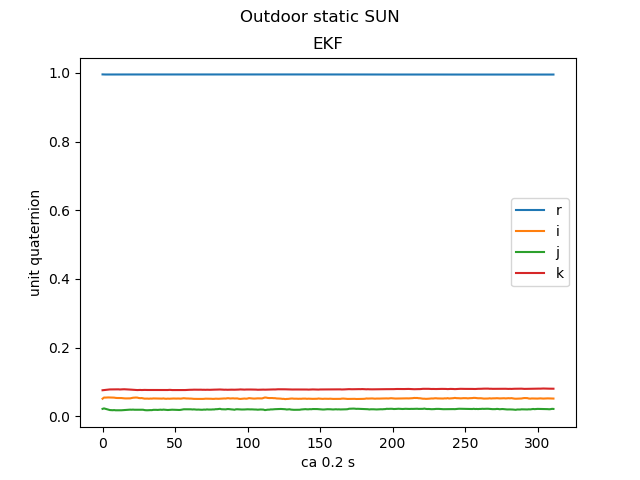
\includegraphics[width=1\columnwidth]{./Pictures/run3OutdoorStaticSUN}
	\caption{Plot of recorded quaternion quaternion for Outdoor test using the PrintSat. Static test with sun}
	\label{fig:Outdoor3RotNoSun}
\end{figure}

\begin{figure}[tbp]
	\centering
	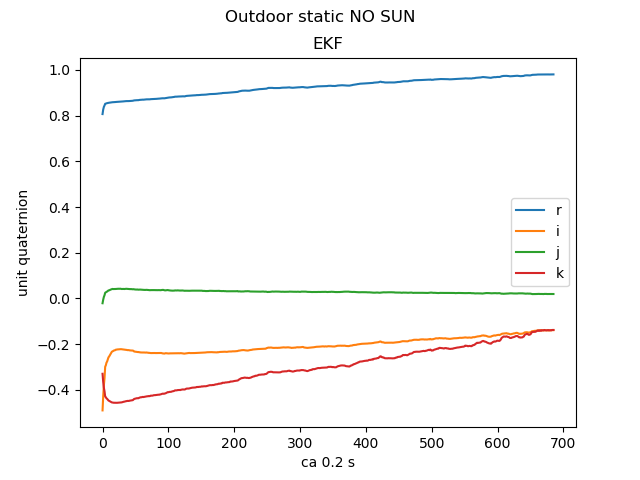
\includegraphics[width=1\columnwidth]{./Pictures/run3OutdoorStaticNOSUN}
	\caption{Plot of recorded quaternion for Outdoor test using the PrintSat. Static with  no sun}
	\label{fig:Outdoor3RotNoSun}
\end{figure}         

Some effort have been put into trying to figure out why this happens. An initial theory is was that it is due to the fact that the EKF is not initialized by the SVD and that it will converge to the right value give enough time. It is just so slow because the initial estimate is so far away from the correct estimate. The problem with this theory is that the ADS seems to work when there is rotation and no sun. In this scenario there is also no SVD initialization, so it seems like the EKF works even with out the SVD initialization. As a part of the future investigation a static Algorithm only test where conducted where the conditions where changed from sun to no sun before it was set back to sun. The results can be seen in \autoref{fig:cdrSunNoSunSun}. The results show that the quaternions stay constant even when there is sun if they have converged to the right values first. This at least indicates that the EKF does not diverge if the quaternions have already converge to the right value. For future investigation the problem have been recreated in simulations. This also indicates that the problem is a problem with the algorithm itself and not the implementation on the satellite or any hardware related issues. 

\begin{figure}[tbp]
	\centering
	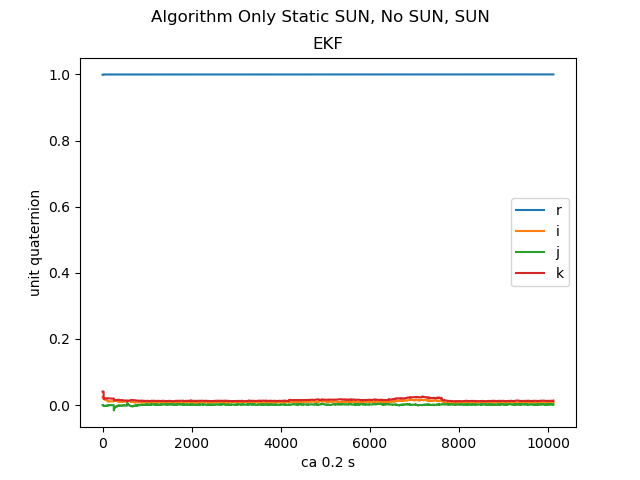
\includegraphics[width=1\columnwidth]{./Pictures/cdrRun1StaticSunEclipsSun}
	\caption{Plot of recorded quaternion for Algorithm only test test using the PrintSat. Static test where the condition are changed from sun to no sun and then back to sun. }
	\label{fig:cdrSunNoSunSun}
\end{figure} 

\subsection{Flight Model}
The test with the FM where limited in scope and mostly to verify that the same behavior that is seen on the PrintSat can be seen on the FM as well. There results from two test shown in \autoref{fig:FMcdrTwoRotSun} and \autoref{fig:FMcdrTwoRotNoSun} show that the results are somewhat consistent with the PrintSat. The overall trend in both is that ADS is preforming reasonably well and the estimated quaternions are able to follow the reference quaternions reasonably well. In \autoref{fig:FMcdrTwoRotSun} the preference is a lot worse than on the PrintSat equivalent test seen in \autoref{fig:cdr3RotSun}. There are this seemingly periodic shifts in the estimated quaternion that was not so viable on the PrintSat. This seems to come from spikes in the sun sensor measurements as you can see in the bottom plot of \autoref{fig:FMcdrTwoRotSun} there is a shift in the estimated quaternion whenever there are spikes in the sun sensor measurement. The spikes in the sun sensor measurements seem to come from when there is a switch in which sun sensor that is being used. The switching comes from a new panel side panel facing the sun. The reason why the spikes in sun sensor measurements are only on the FM and not on the PrintSat is still under investigation, but the working theory is that the spikes comes from the environment. As the FM test was conducted in the integration that is not completely dark while the PrintSat test where done in a complete dark room. 

\begin{figure}[tbp]
	\centering
	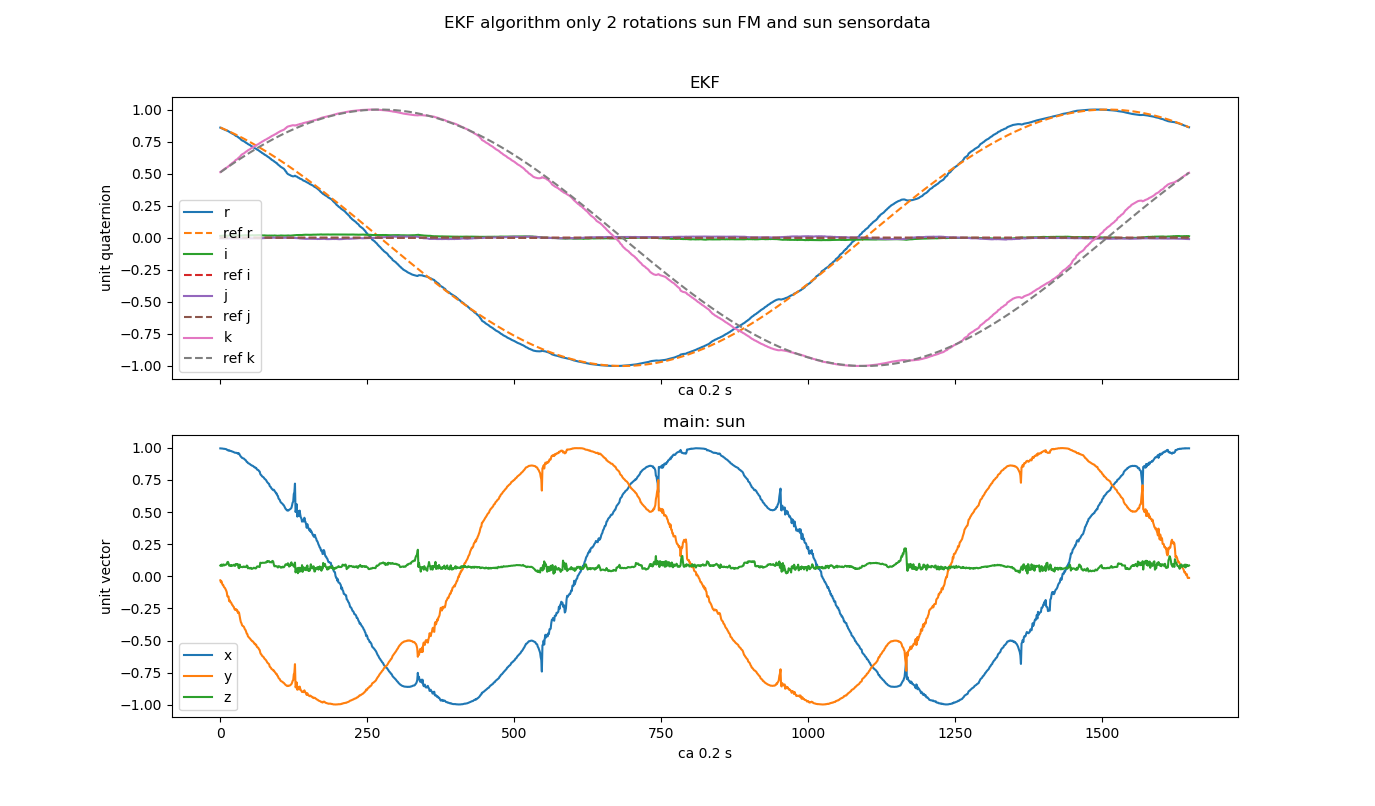
\includegraphics[width=1\columnwidth]{./Pictures/test1EKFandSUN}
	\caption{Plot of recorded quaternion for Algorithm only test test using the FM and the recorded sun sensor measurements. The FM is turned two time on the turntable.}
	\label{fig:FMcdrTwoRotSun}
\end{figure}

\begin{figure}[tbp]
	\centering
	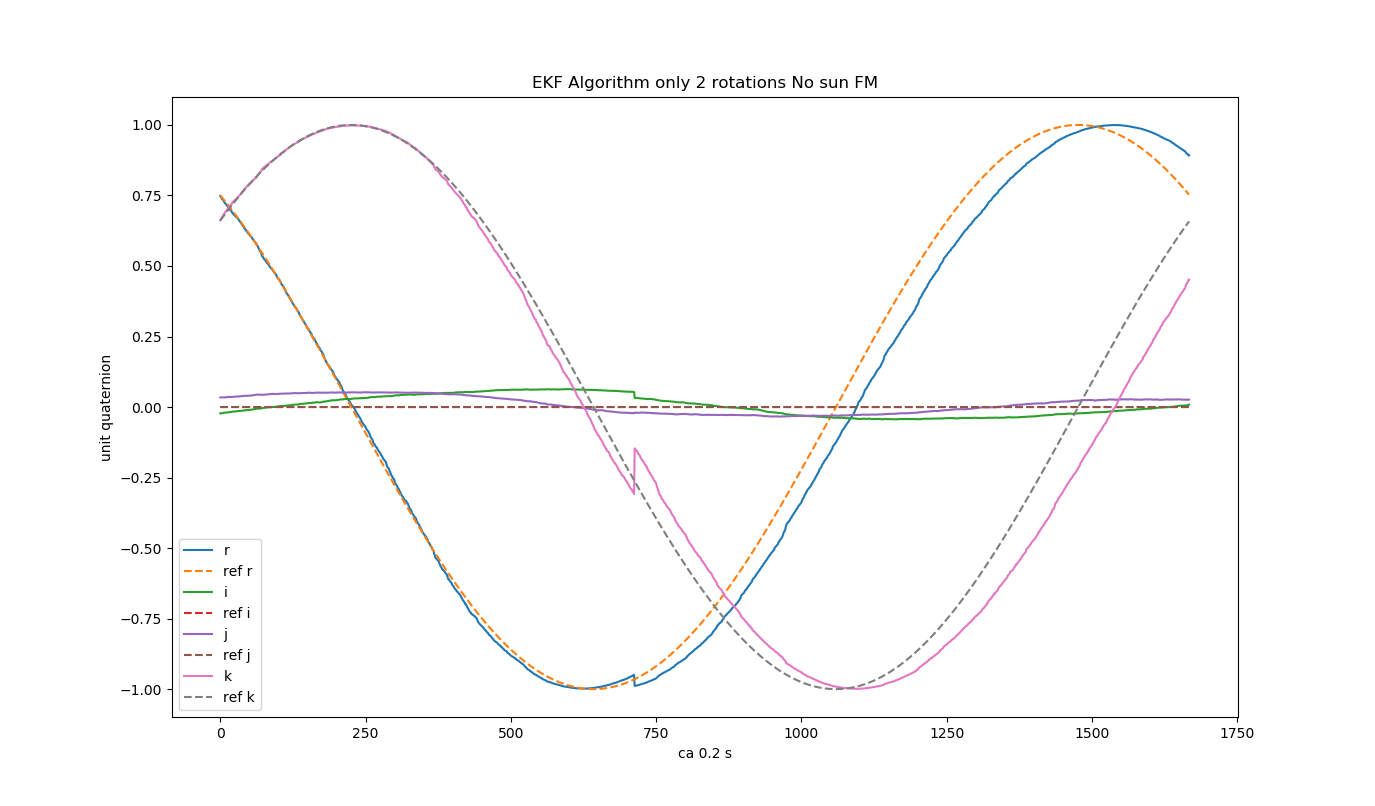
\includegraphics[width=1\columnwidth]{./Pictures/EKF_Algorithm_only_2_rotations_No_sun_FM}
	\caption{Plot of recorded quaternion for Algorithm only test using the FM. The FM is turned two times on the turntable.}
	\label{fig:FMcdrTwoRotNoSun}
\end{figure}   

The one shift that can be seen in \autoref{fig:FMcdrTwoRotNoSun} also comes from when the natural light in the integration room was accepted as a valid sun sensor measurement and therefore used in the EKF cosing the shift. One thing that is interesting to note is that the quaternion does not converge back to the correct estimate but instead follows the reference quaternion with a constant error.     
\fi
